% Drawing 144/05-2 -- folder 144, batch 05, archive page 87 (PDF page 88).
% Transcription: deux sphères reliées par une flèche. À gauche, $X_n$ : pôles $P_\omega$ (haut) et $P_{\omega'}$ (bas), sur l'équateur $R_0$, $Q_{a_0}$, $R_1$ ; méridiens ; le point $P$ près de $P_\omega$, avec les chemins $\alpha$, $\alpha_\rho$ vers $\rho(P)$, $\rho(\alpha)$, et sous l'équateur $\alpha_\sigma$, $\sigma_{a_0}^0(P)$, $\sigma_{a_0}^0(\alpha)$, $\lambda_{a_0}$. À droite, $X_0$ : le pôle $P_+$, le point $\infty$, le segment $[0,1]$ sur l'équateur, les hémisphères $X_0^+$ et $X_0^-$, et le lacet $g_n(\alpha_\rho)$.
% Kind: two spheres X_n -> X_0 with paths and loops. Method 2 (schematic redraw from the facsimile). Status: partial.
% Notes: Each sphere re-read on a tight crop; points placed once and every path drawn to them. Left, X_n: pencil outline and equator; the front of the equator inked from R_0 through Q_{a_0} and R_1 to a fourth point at the right; meridians from P_omega: the solid ones to R_1 and to the right-hand point, the dashed one through Q_{a_0} (lambda_{a_0}, with its arrow up from Q_{a_0}) continuing below the equator to P_omega'. The point P near P_omega with the bold dashed path alpha from P_omega; the double arrow alpha_rho from P to rho(P), and the dashed rho(alpha) from P_omega to rho(P); below the equator the dashed path alpha_sigma from P down and across to sigma^0_{a_0}(P), and sigma^0_{a_0}(alpha) from P_omega' up to it. Right, X_0: pencil outline and equator, the segment [0, 1] inked on the front of the equator, infinity at the back, P_+, X_0^+ and X_0^-, and the loop g_n(alpha_rho): dashed from P_+ down the left, an arrow to the equator, dashed along the back, the double arrow, dashed up the right with an arrowhead back to P_+. The arrow X_n -> X_0 between them. Labels \small. Still differs from the facsimile: the small circled a_0 and the label read K'_{a_0} or alpha'_sigma next to lambda_{a_0} are not drawn (illegible); the short dashed vertical right of lambda_{a_0} is drawn but its role is not clear; the outlines are doubled on the page and drawn once; the arrowheads along the paths are a reading. The text around the figures is not drawn. Redrawn 2026-11-09 (issue 128): to check again. Overlay check 2026-11-13 (issue 147, Claude Opus 5.5): the redraw, rasterised from its TikZ paths, laid over the 300 dpi colour render of the 250 ppi scan with the contrast raised: the paths, meridians, the inked front of the equator, the segment [0, 1] and the arrow between the spheres lie on their ink (88 % of the drawn length within 0.6 unit of ink, no stroke below 70 %). Nothing changed. Still differs, as listed above: the pencil outlines of both spheres are gone over two or three times on the page and drawn once, as ellipses; the small circled a_0 and the label read K'_{a_0} or alpha'_sigma beside lambda_{a_0} stay illegible and are not drawn; the arrowheads along the paths are a reading. Not compiled (no TeX engine in the session).
% Coordinates: 1 unit = 1 mm = 1/100 of the crop width (bbox in page fractions: [0.06, 0.33, 0.68, 0.54]).
% Redrawn by Claude (claude-opus-5-5), issue #73, 2026-11-09; not checked by a human; not compiled (no TeX in the session).
% Checked by Claude (claude-opus-5-5) 2026-11-13 (issue #147): overlay on the 300 dpi colour render of the 250 ppi scan; nothing changed; not compiled (no TeX in the session). Not checked by a human. Status: partial.
% Rights: reproduces part of the work -- behind RENDER_TRANSCRIPTS, never published by itself.
\documentclass[tikz,border=3pt]{standalone}
\usepackage{amsmath,amssymb}
\usetikzlibrary{patterns,arrows.meta}
\tikzset{pencil/.style={black!45}, struck/.style={black!35}, mark/.style={circle,draw,inner sep=1.3pt}, pt/.style={circle,fill,inner sep=0.9pt}, opt/.style={circle,draw,fill=white,inner sep=1.1pt}}
\begin{document}
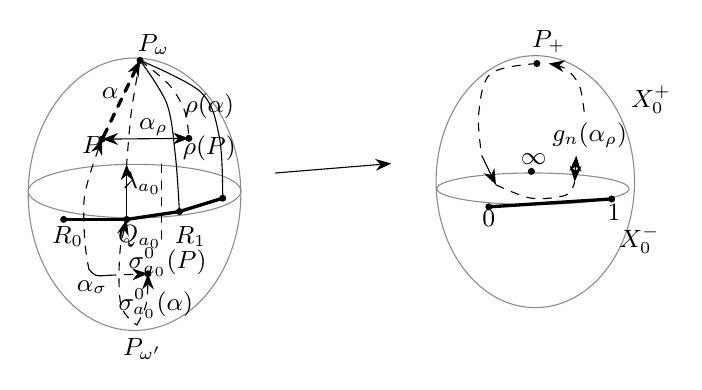
\begin{tikzpicture}[x=1mm,y=1mm,line cap=round,line join=round,font=\scriptsize]
\draw[pencil] (23.4,-25.8) ellipse[x radius=13.5, y radius=17.3];
\draw[pencil] (23.4,-25.4) ellipse[x radius=13.5, y radius=3.4];
\draw[very thick] (14.4,-29) -- (22.4,-29);
\draw[very thick] (22.4,-29) -- (29.1,-28);
\draw[very thick] (29.1,-28) -- (34.6,-26.3);
\draw[dashed,very thick,{Stealth[length=2mm]}-] (24.1,-8.8) -- (19.3,-18.8);
\draw[dashed,{Stealth[length=2mm]}-] plot[smooth, tension=0.55] coordinates {(19.3,-18.8) (18,-22.4) (17,-26.5) (17.1,-31.9) (17.6,-35.3)};
\draw plot[smooth, tension=0.55] coordinates {(17.6,-35.3) (18.5,-36.1) (20,-36.1)};
\draw[dashed,-{Stealth[length=2mm]}] (20,-36.1) -- (25.1,-35.9);
\draw[dashed] plot[smooth, tension=0.55] coordinates {(24.1,-8.8) (23,-15.3) (22.4,-22)};
\draw[-{Stealth[length=2mm]}] (22.4,-29) -- (22.4,-22);
\draw[dashed,{Stealth[length=2mm]}-] plot[smooth, tension=0.55] coordinates {(22.4,-29) (21.5,-33.9) (21.7,-40) (23.7,-42.4)};
\draw[dashed,-{Stealth[length=2mm]}] plot[smooth, tension=0.55] coordinates {(23.7,-42.4) (24.9,-39.7) (25.1,-35.9)};
\draw plot[smooth, tension=0.55] coordinates {(24.1,-8.8) (27.5,-14.3) (28.6,-21) (29.1,-28)};
\draw plot[smooth, tension=0.55] coordinates {(24.1,-8.8) (31.9,-12.9) (34.2,-18.7) (34.6,-26.3)};
\draw[dashed] plot[smooth, tension=0.55] coordinates {(24.1,-8.8) (27.8,-11.9) (29.8,-15.3) (30.3,-18.7)};
\draw[{Stealth[length=2mm]}-{Stealth[length=2mm]}] (19.3,-18.8) -- (30.3,-18.7);
\draw[dashed] (26.8,-22) -- (26.8,-32.2);
\node[pt] at (24.1,-8.8) {};
\node[pt] at (19.3,-18.8) {};
\node[pt] at (30.3,-18.7) {};
\node[pt] at (14.4,-29) {};
\node[pt] at (22.4,-29) {};
\node[pt] at (29.1,-28) {};
\node[pt] at (34.6,-26.3) {};
\node[pt] at (25.1,-35.9) {};
\node[inner sep=1pt] at (25.8,-6.8) {\small $P_\omega$};
\node[inner sep=1pt] at (20.3,-12.9) {\small $\alpha$};
\node[inner sep=1pt] at (18,-19.5) {\small $P$};
\node[inner sep=1pt] at (25.8,-17.3) {\small $\alpha_\rho$};
\node[inner sep=1pt] at (32.9,-14.6) {\small $\rho(\alpha)$};
\node[inner sep=1pt] at (32.9,-20) {\small $\rho(P)$};
\node[inner sep=1pt] at (24.4,-24.4) {\small $\lambda_{a_0}$};
\node[inner sep=1pt] at (14.9,-31.2) {\small $R_0$};
\node[inner sep=1pt] at (24.1,-31.2) {\small $Q_{a_0}$};
\node[inner sep=1pt] at (30.5,-31.2) {\small $R_1$};
\node[inner sep=1pt] at (27.6,-34.4) {\small $\sigma^0_{a_0}(P)$};
\node[inner sep=1pt] at (26.1,-39.7) {\small $\sigma^0_{a_0}(\alpha)$};
\node[inner sep=1pt] at (18,-37.6) {\small $\alpha_\sigma$};
\node[inner sep=1pt] at (24.4,-45.4) {\small $P_{\omega'}$};
\draw[pencil] (74.3,-24.2) ellipse[x radius=12.6, y radius=16];
\draw[pencil] (74,-25.1) ellipse[x radius=12.2, y radius=2];
\draw[very thick] (68.4,-27.4) -- (84,-26.4);
\draw[dashed] plot[smooth, tension=0.55] coordinates {(74.5,-9.2) (68.6,-10.5) (67.1,-15.7) (67.5,-20.9)};
\draw[-{Stealth[length=2mm]}] (67.5,-20.9) -- (69.3,-24.6);
\draw[dashed] plot[smooth, tension=0.55] coordinates {(69.3,-24.6) (73.8,-26.3) (78.2,-25.9) (79.3,-24.2)};
\draw[{Stealth[length=2mm]}-{Stealth[length=2mm]}] (79.3,-24.2) -- (79.5,-20.9);
\draw[dashed,-{Stealth[length=2mm]}] plot[smooth, tension=0.55] coordinates {(80.5,-15.3) (79.9,-12) (78.2,-9.9) (76,-9.2)};
\node[pt] at (74.5,-9.2) {};
\node[pt] at (68.4,-27.4) {};
\node[pt] at (84,-26.4) {};
\node[pt] at (73.8,-22.9) {};
\node[inner sep=1pt] at (76,-6.4) {\small $P_+$};
\node[inner sep=1pt] at (74.1,-21.4) {\small $\infty$};
\node[inner sep=1pt] at (68.4,-28.9) {\small $0$};
\node[inner sep=1pt] at (84.3,-28.1) {\small $1$};
\node[inner sep=1pt] at (81.2,-18.3) {\small $g_n(\alpha_\rho)$};
\node[inner sep=1pt] at (89,-13.8) {\small $X_0^+$};
\node[inner sep=1pt] at (87.5,-31.6) {\small $X_0^-$};
\draw[-{Stealth[length=2mm]}] (41.3,-23.1) -- (56,-21.9);
\end{tikzpicture}
\end{document}
